% Options for packages loaded elsewhere
\PassOptionsToPackage{unicode}{hyperref}
\PassOptionsToPackage{hyphens}{url}
%
\documentclass[
]{article}
\usepackage{amsmath,amssymb}
\usepackage{iftex}
\ifPDFTeX
  \usepackage[T1]{fontenc}
  \usepackage[utf8]{inputenc}
  \usepackage{textcomp} % provide euro and other symbols
\else % if luatex or xetex
  \usepackage{unicode-math} % this also loads fontspec
  \defaultfontfeatures{Scale=MatchLowercase}
  \defaultfontfeatures[\rmfamily]{Ligatures=TeX,Scale=1}
\fi
\usepackage{lmodern}
\ifPDFTeX\else
  % xetex/luatex font selection
\fi
% Use upquote if available, for straight quotes in verbatim environments
\IfFileExists{upquote.sty}{\usepackage{upquote}}{}
\IfFileExists{microtype.sty}{% use microtype if available
  \usepackage[]{microtype}
  \UseMicrotypeSet[protrusion]{basicmath} % disable protrusion for tt fonts
}{}
\makeatletter
\@ifundefined{KOMAClassName}{% if non-KOMA class
  \IfFileExists{parskip.sty}{%
    \usepackage{parskip}
  }{% else
    \setlength{\parindent}{0pt}
    \setlength{\parskip}{6pt plus 2pt minus 1pt}}
}{% if KOMA class
  \KOMAoptions{parskip=half}}
\makeatother
\usepackage{xcolor}
\usepackage[margin=1in]{geometry}
\usepackage{color}
\usepackage{fancyvrb}
\newcommand{\VerbBar}{|}
\newcommand{\VERB}{\Verb[commandchars=\\\{\}]}
\DefineVerbatimEnvironment{Highlighting}{Verbatim}{commandchars=\\\{\}}
% Add ',fontsize=\small' for more characters per line
\usepackage{framed}
\definecolor{shadecolor}{RGB}{248,248,248}
\newenvironment{Shaded}{\begin{snugshade}}{\end{snugshade}}
\newcommand{\AlertTok}[1]{\textcolor[rgb]{0.94,0.16,0.16}{#1}}
\newcommand{\AnnotationTok}[1]{\textcolor[rgb]{0.56,0.35,0.01}{\textbf{\textit{#1}}}}
\newcommand{\AttributeTok}[1]{\textcolor[rgb]{0.13,0.29,0.53}{#1}}
\newcommand{\BaseNTok}[1]{\textcolor[rgb]{0.00,0.00,0.81}{#1}}
\newcommand{\BuiltInTok}[1]{#1}
\newcommand{\CharTok}[1]{\textcolor[rgb]{0.31,0.60,0.02}{#1}}
\newcommand{\CommentTok}[1]{\textcolor[rgb]{0.56,0.35,0.01}{\textit{#1}}}
\newcommand{\CommentVarTok}[1]{\textcolor[rgb]{0.56,0.35,0.01}{\textbf{\textit{#1}}}}
\newcommand{\ConstantTok}[1]{\textcolor[rgb]{0.56,0.35,0.01}{#1}}
\newcommand{\ControlFlowTok}[1]{\textcolor[rgb]{0.13,0.29,0.53}{\textbf{#1}}}
\newcommand{\DataTypeTok}[1]{\textcolor[rgb]{0.13,0.29,0.53}{#1}}
\newcommand{\DecValTok}[1]{\textcolor[rgb]{0.00,0.00,0.81}{#1}}
\newcommand{\DocumentationTok}[1]{\textcolor[rgb]{0.56,0.35,0.01}{\textbf{\textit{#1}}}}
\newcommand{\ErrorTok}[1]{\textcolor[rgb]{0.64,0.00,0.00}{\textbf{#1}}}
\newcommand{\ExtensionTok}[1]{#1}
\newcommand{\FloatTok}[1]{\textcolor[rgb]{0.00,0.00,0.81}{#1}}
\newcommand{\FunctionTok}[1]{\textcolor[rgb]{0.13,0.29,0.53}{\textbf{#1}}}
\newcommand{\ImportTok}[1]{#1}
\newcommand{\InformationTok}[1]{\textcolor[rgb]{0.56,0.35,0.01}{\textbf{\textit{#1}}}}
\newcommand{\KeywordTok}[1]{\textcolor[rgb]{0.13,0.29,0.53}{\textbf{#1}}}
\newcommand{\NormalTok}[1]{#1}
\newcommand{\OperatorTok}[1]{\textcolor[rgb]{0.81,0.36,0.00}{\textbf{#1}}}
\newcommand{\OtherTok}[1]{\textcolor[rgb]{0.56,0.35,0.01}{#1}}
\newcommand{\PreprocessorTok}[1]{\textcolor[rgb]{0.56,0.35,0.01}{\textit{#1}}}
\newcommand{\RegionMarkerTok}[1]{#1}
\newcommand{\SpecialCharTok}[1]{\textcolor[rgb]{0.81,0.36,0.00}{\textbf{#1}}}
\newcommand{\SpecialStringTok}[1]{\textcolor[rgb]{0.31,0.60,0.02}{#1}}
\newcommand{\StringTok}[1]{\textcolor[rgb]{0.31,0.60,0.02}{#1}}
\newcommand{\VariableTok}[1]{\textcolor[rgb]{0.00,0.00,0.00}{#1}}
\newcommand{\VerbatimStringTok}[1]{\textcolor[rgb]{0.31,0.60,0.02}{#1}}
\newcommand{\WarningTok}[1]{\textcolor[rgb]{0.56,0.35,0.01}{\textbf{\textit{#1}}}}
\usepackage{graphicx}
\makeatletter
\newsavebox\pandoc@box
\newcommand*\pandocbounded[1]{% scales image to fit in text height/width
  \sbox\pandoc@box{#1}%
  \Gscale@div\@tempa{\textheight}{\dimexpr\ht\pandoc@box+\dp\pandoc@box\relax}%
  \Gscale@div\@tempb{\linewidth}{\wd\pandoc@box}%
  \ifdim\@tempb\p@<\@tempa\p@\let\@tempa\@tempb\fi% select the smaller of both
  \ifdim\@tempa\p@<\p@\scalebox{\@tempa}{\usebox\pandoc@box}%
  \else\usebox{\pandoc@box}%
  \fi%
}
% Set default figure placement to htbp
\def\fps@figure{htbp}
\makeatother
\setlength{\emergencystretch}{3em} % prevent overfull lines
\providecommand{\tightlist}{%
  \setlength{\itemsep}{0pt}\setlength{\parskip}{0pt}}
\setcounter{secnumdepth}{-\maxdimen} % remove section numbering
\usepackage{bookmark}
\IfFileExists{xurl.sty}{\usepackage{xurl}}{} % add URL line breaks if available
\urlstyle{same}
\hypersetup{
  pdftitle={The relationship between unemployment and crime in the Netherlands},
  pdfauthor={Romeo Schoonderbeek, 2868407 Paul Claessens, 2859603 Furkan Kadir Öztürk, 2852640 Serena Kula 2856584 Bjorn Smit 2812968 Lia Seo 2841955},
  hidelinks,
  pdfcreator={LaTeX via pandoc}}

\title{The relationship between unemployment and crime in the
Netherlands}
\author{Romeo Schoonderbeek, 2868407 Paul Claessens, 2859603 Furkan
Kadir Öztürk, 2852640 Serena Kula 2856584 Bjorn Smit 2812968 Lia Seo
2841955}
\date{2025-06-24}

\begin{document}
\maketitle

\section{Set-up your environment}\label{set-up-your-environment}

\begin{Shaded}
\begin{Highlighting}[]
\FunctionTok{require}\NormalTok{(tidyverse)}
\end{Highlighting}
\end{Shaded}

\begin{verbatim}
## Loading required package: tidyverse
\end{verbatim}

\begin{verbatim}
## -- Attaching core tidyverse packages ------------------------ tidyverse 2.0.0 --
## v dplyr     1.1.4     v readr     2.1.5
## v forcats   1.0.0     v stringr   1.5.1
## v ggplot2   3.5.2     v tibble    3.3.0
## v lubridate 1.9.4     v tidyr     1.3.1
## v purrr     1.0.4     
## -- Conflicts ------------------------------------------ tidyverse_conflicts() --
## x dplyr::filter() masks stats::filter()
## x dplyr::lag()    masks stats::lag()
## i Use the conflicted package (<http://conflicted.r-lib.org/>) to force all conflicts to become errors
\end{verbatim}

\begin{Shaded}
\begin{Highlighting}[]
\FunctionTok{require}\NormalTok{(cbsodataR)}
\end{Highlighting}
\end{Shaded}

\begin{verbatim}
## Loading required package: cbsodataR
\end{verbatim}

\begin{Shaded}
\begin{Highlighting}[]
\FunctionTok{require}\NormalTok{(sf)}
\end{Highlighting}
\end{Shaded}

\begin{verbatim}
## Loading required package: sf
## Linking to GEOS 3.13.0, GDAL 3.5.3, PROJ 9.5.1; sf_use_s2() is TRUE
\end{verbatim}

\section{Part 1 - Identify a Social
Problem}\label{part-1---identify-a-social-problem}

\subsection{1.1 Describe the Social
Problem}\label{describe-the-social-problem}

Our Social problem is to look at the relation between crime and
unemployment, since these are often believed to be related with each
other. Unemployment can cause financial stress and social exclusion,
these factors can lead to criminal activity. Criminal records can also
lower the chances of being accepted for a job, which makes criminal
activity an easier option. Why this is a relevant issue, even though
crime rates in the Netherlands have seen a steady decline. Financial and
online crime are relatively growing (Nieuws Sociaal en Groen, 2023).
Whilst youth unemployment remains a prominent issue in vulnerable
communities. Understanding the relationship between unemployment and
crime is highly important for the design of social and economic
policies. A study by Verbruggen(2014), reviewed by Fischer(2015) shows a
critical perspective on the relationship between crime and unemployment.
It shows that employment is generally associated with lower crime rates,
however it also shows that unemployment doesn't necessarily lead to more
crime. Whilst Verbruggen (2014) gives a good insight into the vulnerable
Dutch population, broader analyses of this problem are still very
limited. How structural shifts affect this relationship for example.
Additionally, the understanding of spatial and subgroup variations in
the Netherlands are also limited. We aim to contribute towards the
limited understanding of the special and subgroup variations.

\section{Part 2 - Data Sourcing}\label{part-2---data-sourcing}

\subsection{2.1 Load in the data}\label{load-in-the-data}

\begin{Shaded}
\begin{Highlighting}[]
\CommentTok{\# province level}
\NormalTok{DS\_Panel\_Unemployment }\OtherTok{\textless{}{-}} \FunctionTok{read.csv}\NormalTok{(}\StringTok{"data/raw\_data/unemployment\_data\_transform.csv"}\NormalTok{)}
\NormalTok{DS\_Panel\_Crime }\OtherTok{\textless{}{-}} \FunctionTok{read.csv}\NormalTok{(}\StringTok{"data/raw\_data/panel\_data\_crime.csv"}\NormalTok{)}
\NormalTok{DS\_Population }\OtherTok{\textless{}{-}} \FunctionTok{read.csv}\NormalTok{(}\StringTok{"data/raw\_data/population\_data.csv"}\NormalTok{)}
\NormalTok{area\_data\_working }\OtherTok{\textless{}{-}} \FunctionTok{read.csv}\NormalTok{(}\StringTok{"data/raw\_data/area\_data.csv"}\NormalTok{)}

\CommentTok{\# aggragate}
\NormalTok{agg\_unemployment }\OtherTok{\textless{}{-}} \FunctionTok{read.csv}\NormalTok{(}\StringTok{"data/raw\_data/aggragate\_total\_unemployment.csv"}\NormalTok{)}
\NormalTok{agg\_crime }\OtherTok{\textless{}{-}} \FunctionTok{read.csv}\NormalTok{(}\StringTok{"data/raw\_data/aggragate\_total\_crime.csv"}\NormalTok{)}
\NormalTok{agg\_population }\OtherTok{\textless{}{-}} \FunctionTok{read.csv}\NormalTok{(}\StringTok{"data/raw\_data/population\_data\_raw.csv"}\NormalTok{)}

\CommentTok{\# subpopulation}
\NormalTok{criminaliteit\_per\_leeftijd }\OtherTok{\textless{}{-}} \FunctionTok{read.csv}\NormalTok{(}\StringTok{"data/raw\_data/criminaliteit\_per\_leeftijd.csv"}\NormalTok{) }

\NormalTok{unemployment\_age }\OtherTok{\textless{}{-}} \FunctionTok{read.csv}\NormalTok{(}\StringTok{"data/raw\_data/unemployment\_per\_age.csv"}\NormalTok{) }
\end{Highlighting}
\end{Shaded}

\subsection{2.2 Provide a short summary of the
dataset's}\label{provide-a-short-summary-of-the-datasets}

The data sets are categorized within 3 categories: province level,
aggregate and sub population. Since our topic is the relation between
crime and unemployment in the Netherlands, these datasets are very
suitable. The datasets do not only provide the crime and unemployment
data for the Netherlands it self but also on a provincial level and age
category, which allows for spatial variation and subpopulation analysis.
The main variables used are unemployment rates - total unemployed
working population/working population*100 - and amount of crimes
registered per year. Since the data sets are classified as panel data
sets, unemployment and crime can be compared to each year. Population
data sets are used to convert total crime to crime per capita, which
allows for population control per province. CBS measures unemployment by
surveying 20000 Dutch people of working age who actively seek
employment, but are not employed. Population data each year is measured
by Basis regristartie personen. And crime data originates from data
gathered by the Dutch police.

\subsection{2.3 limitations}\label{limitations}

For crime statistics, only crimes that are registered are accounted for,
there are also crimes that have not been reported and thus not counted
in the datasets. Furthemore, the data does not distinguish if
perpratrators were unemployed. So the validity of the conclusions draw
from this data can never be fully verified. Additionally, people
reported as unemployed might do undeclared work.

\section{Part 3 - Quantifying}\label{part-3---quantifying}

\subsection{3.1 Data cleaning}\label{data-cleaning}

CBS datasets already come in panel data form. Data cleaning will include
removing unnecessary rows and columns, adjusting data frames and merging
data sets. 3 main data sets are used. Province panel data, aggregate
panel data and data sets used for sub population analysis.Futhermore,
certain entries within data sets have to be converted to numerics.
Finally column names are given to make the data sets more structured and
formal.

\begin{Shaded}
\begin{Highlighting}[]
\CommentTok{\# province panel data cleaning}

\NormalTok{merged\_data }\OtherTok{\textless{}{-}} \FunctionTok{cbind}\NormalTok{(DS\_Panel\_Unemployment, DS\_Panel\_Crime [, }\DecValTok{5}\NormalTok{])}

\NormalTok{merged\_data }\OtherTok{\textless{}{-}}\FunctionTok{cbind}\NormalTok{(merged\_data, DS\_Population [, }\DecValTok{4}\NormalTok{])}

\NormalTok{merged\_data }\OtherTok{\textless{}{-}}\NormalTok{ merged\_data [, }\SpecialCharTok{{-}}\FunctionTok{c}\NormalTok{(}\DecValTok{1}\NormalTok{)] }
\FunctionTok{colnames}\NormalTok{(merged\_data) }\OtherTok{\textless{}{-}} \FunctionTok{c}\NormalTok{(}\StringTok{"Year"}\NormalTok{, }\StringTok{"province"}\NormalTok{, }\StringTok{"Unemployment\_Rate"}\NormalTok{, }\StringTok{"total\_Crimes"}\NormalTok{, }\StringTok{"Population"}\NormalTok{)}

\NormalTok{merged\_data }\OtherTok{\textless{}{-}} \FunctionTok{mutate}\NormalTok{(merged\_data, }\AttributeTok{crimes\_per\_capita =}\NormalTok{ (total\_Crimes}\SpecialCharTok{/}\NormalTok{Population)}\SpecialCharTok{*}\DecValTok{100}\NormalTok{)}

\FunctionTok{write.csv}\NormalTok{(merged\_data, }\StringTok{"data/working\_data/merged\_panel\_data\_final.csv"}\NormalTok{)}

\NormalTok{area\_data\_working }\OtherTok{\textless{}{-}} \FunctionTok{read.csv}\NormalTok{(}\StringTok{"data/raw\_data/area\_data.csv"}\NormalTok{)}

\FunctionTok{colnames}\NormalTok{(area\_data\_working) }\OtherTok{=} \FunctionTok{c}\NormalTok{(}\StringTok{"X"}\NormalTok{, }\StringTok{"province"}\NormalTok{, }\StringTok{"Area(KM2)"}\NormalTok{)}

\NormalTok{area\_data\_working }\OtherTok{\textless{}{-}}\NormalTok{ area\_data\_working[}\DecValTok{6}\SpecialCharTok{:}\DecValTok{17}\NormalTok{ ,]}

\NormalTok{area\_data\_working[[}\DecValTok{3}\NormalTok{]]  }\OtherTok{=} \FunctionTok{as.numeric}\NormalTok{(area\_data\_working[[}\DecValTok{3}\NormalTok{]])}

\NormalTok{area\_data\_working[, }\DecValTok{3}\NormalTok{] }\OtherTok{=}\NormalTok{ area\_data\_working[, }\DecValTok{3}\NormalTok{]}\SpecialCharTok{/} \DecValTok{100}

\NormalTok{flevoland }\OtherTok{\textless{}{-}} \FunctionTok{data.frame}\NormalTok{(}\AttributeTok{name =} \StringTok{"Flevoland"}\NormalTok{, }\AttributeTok{value =} \DecValTok{1417}\NormalTok{ )}
\FunctionTok{colnames}\NormalTok{(flevoland) }\OtherTok{=} \FunctionTok{c}\NormalTok{(}\StringTok{"province"}\NormalTok{, }\StringTok{"Area(KM2)"}\NormalTok{)}

\NormalTok{area\_data\_working }\OtherTok{\textless{}{-}} \FunctionTok{bind\_rows}\NormalTok{(}
\NormalTok{  area\_data\_working[}\DecValTok{1}\SpecialCharTok{:}\DecValTok{5}\NormalTok{, ], flevoland,  }
\NormalTok{  area\_data\_working[}\DecValTok{6}\SpecialCharTok{:}\FunctionTok{nrow}\NormalTok{(area\_data\_working), ]}
\NormalTok{)}
\end{Highlighting}
\end{Shaded}

\begin{verbatim}
## New names:
## New names:
## * `` -> `...4`
## * `` -> `...5`
## * `` -> `...6`
\end{verbatim}

\begin{Shaded}
\begin{Highlighting}[]
\NormalTok{area\_data\_working }\OtherTok{\textless{}{-}}\NormalTok{ area\_data\_working }\SpecialCharTok{\%\textgreater{}\%}
  \FunctionTok{slice}\NormalTok{(}\FunctionTok{rep}\NormalTok{(}\DecValTok{1}\SpecialCharTok{:}\FunctionTok{n}\NormalTok{(), }\AttributeTok{each =} \DecValTok{12}\NormalTok{))}

\NormalTok{merged\_panel\_data\_final }\OtherTok{\textless{}{-}} \FunctionTok{cbind}\NormalTok{(merged\_data, area\_data\_working[, }\DecValTok{3}\NormalTok{])}

\FunctionTok{colnames}\NormalTok{(merged\_panel\_data\_final) }\OtherTok{\textless{}{-}} \FunctionTok{c}\NormalTok{(}\StringTok{"year"}\NormalTok{, }\StringTok{"province"}\NormalTok{, }\StringTok{"unemployment\_rate"}\NormalTok{, }\StringTok{"total\_crimes"}\NormalTok{, }\StringTok{"population"}\NormalTok{, }\StringTok{"crimes\_per\_capita"}\NormalTok{, }\StringTok{"area\_km2"}\NormalTok{)}
\end{Highlighting}
\end{Shaded}

\begin{Shaded}
\begin{Highlighting}[]
\CommentTok{\# aggregate data cleaning}

\NormalTok{agg\_unemployment }\OtherTok{\textless{}{-}}\NormalTok{ agg\_unemployment[}\SpecialCharTok{{-}}\FunctionTok{c}\NormalTok{(}\DecValTok{51}\NormalTok{,}\DecValTok{52}\NormalTok{) ,]}
\NormalTok{agg\_unemployment }\OtherTok{\textless{}{-}}\NormalTok{ agg\_unemployment[, }\SpecialCharTok{{-}}\DecValTok{1}\NormalTok{]}

\NormalTok{agg\_crime }\OtherTok{\textless{}{-}}\NormalTok{ agg\_crime[}\SpecialCharTok{{-}}\DecValTok{82}\NormalTok{ , ]}
\NormalTok{agg\_crime }\OtherTok{\textless{}{-}}\NormalTok{ agg\_crime[}\SpecialCharTok{{-}}\FunctionTok{c}\NormalTok{(}\DecValTok{1}\SpecialCharTok{:}\DecValTok{31}\NormalTok{) ,]}
\NormalTok{agg\_crime }\OtherTok{\textless{}{-}}\NormalTok{ agg\_crime[, }\SpecialCharTok{{-}}\DecValTok{1}\NormalTok{]}

\FunctionTok{colnames}\NormalTok{(agg\_unemployment) }\OtherTok{=} \FunctionTok{c}\NormalTok{(}\StringTok{"year"}\NormalTok{, }\StringTok{"unemployment"}\NormalTok{)}
\FunctionTok{colnames}\NormalTok{(agg\_crime) }\OtherTok{=} \FunctionTok{c}\NormalTok{(}\StringTok{"year"}\NormalTok{, }\StringTok{"total\_crimes"}\NormalTok{)}

\NormalTok{agg\_merged }\OtherTok{\textless{}{-}} \FunctionTok{cbind}\NormalTok{(agg\_unemployment, agg\_crime[, }\DecValTok{2}\NormalTok{])}

\FunctionTok{colnames}\NormalTok{(agg\_merged) }\OtherTok{=} \FunctionTok{c}\NormalTok{(}\StringTok{"year"}\NormalTok{, }\StringTok{"unemployment"}\NormalTok{, }\StringTok{"total\_crime"}\NormalTok{)}

\NormalTok{agg\_merged }\OtherTok{\textless{}{-}}\NormalTok{ agg\_merged }\SpecialCharTok{\%\textgreater{}\%}
  \FunctionTok{mutate}\NormalTok{(}\AttributeTok{total\_crime =} \FunctionTok{as.numeric}\NormalTok{(total\_crime)) }\SpecialCharTok{\%\textgreater{}\%}
  \FunctionTok{mutate}\NormalTok{(}\AttributeTok{year =} \FunctionTok{as.numeric}\NormalTok{(year))}

\FunctionTok{str}\NormalTok{(agg\_merged)}
\end{Highlighting}
\end{Shaded}

\begin{verbatim}
## 'data.frame':    50 obs. of  3 variables:
##  $ year        : num  1975 1976 1977 1978 1979 ...
##  $ unemployment: num  3.5 4.2 4.3 4.2 4.1 4.3 5.7 8 9.6 9.6 ...
##  $ total_crime : num  486670 564025 590880 612370 668235 ...
\end{verbatim}

\begin{Shaded}
\begin{Highlighting}[]
\NormalTok{agg\_population }\OtherTok{\textless{}{-}}\NormalTok{agg\_population[, }\SpecialCharTok{{-}}\DecValTok{4}\NormalTok{]}
\NormalTok{agg\_population }\OtherTok{\textless{}{-}}\NormalTok{ agg\_population[, }\SpecialCharTok{{-}}\DecValTok{1}\NormalTok{]}
\NormalTok{agg\_population }\OtherTok{\textless{}{-}}\NormalTok{ agg\_population[}\SpecialCharTok{{-}}\FunctionTok{c}\NormalTok{(}\DecValTok{1}\SpecialCharTok{:}\DecValTok{75}\NormalTok{) ,]}

\NormalTok{agg\_merged }\OtherTok{\textless{}{-}} \FunctionTok{cbind}\NormalTok{(agg\_merged, agg\_population[, }\DecValTok{2}\NormalTok{])}

\FunctionTok{colnames}\NormalTok{(agg\_merged) }\OtherTok{=} \FunctionTok{c}\NormalTok{(}\StringTok{"year"}\NormalTok{, }\StringTok{"unemployment"}\NormalTok{, }\StringTok{"total\_crime"}\NormalTok{, }\StringTok{"population"}\NormalTok{)}
\end{Highlighting}
\end{Shaded}

\begin{Shaded}
\begin{Highlighting}[]
\CommentTok{\# subpopulation}

\NormalTok{crime2021 }\OtherTok{\textless{}{-}}\NormalTok{ criminaliteit\_per\_leeftijd }\SpecialCharTok{\%\textgreater{}\%} \FunctionTok{filter}\NormalTok{(Perioden }\SpecialCharTok{==} \StringTok{"2021"}\NormalTok{)}

\NormalTok{crime2021 }\OtherTok{\textless{}{-}}\NormalTok{ crime2021 }\SpecialCharTok{\%\textgreater{}\%} \FunctionTok{filter}\NormalTok{(Geboorteland }\SpecialCharTok{==} \StringTok{"Totaal"}\NormalTok{)}

\NormalTok{crime2021 }\OtherTok{\textless{}{-}}\NormalTok{ crime2021[, }\SpecialCharTok{{-}}\FunctionTok{c}\NormalTok{(}\DecValTok{1}\SpecialCharTok{:}\DecValTok{2}\NormalTok{, }\DecValTok{4}\SpecialCharTok{:}\DecValTok{8}\NormalTok{)]}

\FunctionTok{colnames}\NormalTok{(crime2021) }\OtherTok{\textless{}{-}} \FunctionTok{c}\NormalTok{(}\StringTok{"Age"}\NormalTok{, }\StringTok{"Crime"}\NormalTok{)}

\NormalTok{crime2021}\SpecialCharTok{$}\NormalTok{Crime }\OtherTok{=}\NormalTok{ (crime2021}\SpecialCharTok{$}\NormalTok{Crime}\SpecialCharTok{/}\DecValTok{10000}\NormalTok{)}\SpecialCharTok{*}\DecValTok{100}

\NormalTok{unemployment\_age }\OtherTok{\textless{}{-}} \FunctionTok{read.csv}\NormalTok{(}\StringTok{"data/raw\_data/unemployment\_per\_age.csv"}\NormalTok{)}

\NormalTok{unemployment\_age }\OtherTok{\textless{}{-}}\NormalTok{ unemployment\_age[}\SpecialCharTok{{-}}\FunctionTok{c}\NormalTok{(}\DecValTok{1}\SpecialCharTok{:}\DecValTok{6}\NormalTok{, }\DecValTok{19}\NormalTok{) ,]}

\NormalTok{unemployment\_age }\OtherTok{\textless{}{-}}\NormalTok{ unemployment\_age[, }\SpecialCharTok{{-}}\DecValTok{1}\NormalTok{]}

\FunctionTok{colnames}\NormalTok{(unemployment\_age) }\OtherTok{=} \FunctionTok{c}\NormalTok{(}\StringTok{"Age"}\NormalTok{, }\StringTok{"Unemployment"}\NormalTok{)}

\NormalTok{unemployment\_age}\SpecialCharTok{$}\NormalTok{Unemployment }\OtherTok{\textless{}{-}} \FunctionTok{gsub}\NormalTok{(}\StringTok{","}\NormalTok{, }\StringTok{"."}\NormalTok{, unemployment\_age}\SpecialCharTok{$}\NormalTok{Unemployment)}

\NormalTok{unemployment\_age}\SpecialCharTok{$}\NormalTok{Unemployment }\OtherTok{\textless{}{-}} \FunctionTok{as.numeric}\NormalTok{(unemployment\_age}\SpecialCharTok{$}\NormalTok{Unemployment)}
\end{Highlighting}
\end{Shaded}

\subsection{3.2 Generate necessary
variables}\label{generate-necessary-variables}

Variable 1 and 2 (Crimes per capita and population density)

\begin{Shaded}
\begin{Highlighting}[]
\NormalTok{agg\_merged }\OtherTok{\textless{}{-}}\NormalTok{ agg\_merged }\SpecialCharTok{\%\textgreater{}\%}
  \FunctionTok{mutate}\NormalTok{(}\AttributeTok{crime\_per\_capita =}\NormalTok{ (total\_crime}\SpecialCharTok{/}\NormalTok{population)}\SpecialCharTok{*}\DecValTok{100}\NormalTok{)}

\NormalTok{merged\_panel\_data\_final }\OtherTok{\textless{}{-}} \FunctionTok{mutate}\NormalTok{(merged\_panel\_data\_final, }\AttributeTok{poplation\_density =}\NormalTok{ population}\SpecialCharTok{/}\NormalTok{area\_km2)}
\end{Highlighting}
\end{Shaded}

Variable 3 Age categories

\begin{Shaded}
\begin{Highlighting}[]
\NormalTok{crime2021}\SpecialCharTok{$}\NormalTok{Age }\OtherTok{\textless{}{-}} \FunctionTok{ifelse}\NormalTok{(crime2021}\SpecialCharTok{$}\NormalTok{Age }\SpecialCharTok{\%in\%} \FunctionTok{c}\NormalTok{(}\StringTok{"12 tot 18 jaar"}\NormalTok{, }\StringTok{"18 tot 23 jaar"}\NormalTok{),}
                                     \StringTok{"Youth (12–23)"}\NormalTok{, }\StringTok{"Adult+ (23+)"}\NormalTok{)}

\NormalTok{unemployment\_age}\SpecialCharTok{$}\NormalTok{Age }\OtherTok{\textless{}{-}} \FunctionTok{ifelse}\NormalTok{(unemployment\_age}\SpecialCharTok{$}\NormalTok{Age }\SpecialCharTok{\%in\%} \FunctionTok{c}\NormalTok{(}\StringTok{"15 tot 20 jaar"}\NormalTok{, }\StringTok{"20 tot 25 jaar"}\NormalTok{),}
                             \StringTok{"Youth (15{-}25)"}\NormalTok{, }\StringTok{"Adult (25+)"}\NormalTok{)}
\end{Highlighting}
\end{Shaded}

\subsection{3.3 Visualize temporal
variation}\label{visualize-temporal-variation}

\begin{Shaded}
\begin{Highlighting}[]
\NormalTok{pivot\_agg\_data }\OtherTok{\textless{}{-}}\NormalTok{ agg\_merged }\SpecialCharTok{\%\textgreater{}\%}
  \FunctionTok{pivot\_longer}\NormalTok{(}\AttributeTok{cols =} \FunctionTok{c}\NormalTok{(unemployment, crime\_per\_capita), }\AttributeTok{names\_to =} \StringTok{"variable"}\NormalTok{, }\AttributeTok{values\_to =} \StringTok{"value"}\NormalTok{)}

\FunctionTok{ggplot}\NormalTok{(pivot\_agg\_data, }\FunctionTok{aes}\NormalTok{(}\AttributeTok{x =}\NormalTok{ year, }\AttributeTok{y =}\NormalTok{ value, }\AttributeTok{colour =}\NormalTok{ variable )) }\SpecialCharTok{+}
  \FunctionTok{geom\_line}\NormalTok{() }\SpecialCharTok{+}
  \FunctionTok{labs}\NormalTok{(}\AttributeTok{title =} \StringTok{"aggragate crime and unemployment through time"}\NormalTok{, }\AttributeTok{x =} \StringTok{"year"}\NormalTok{, }\AttributeTok{y =} \StringTok{"variable"}\NormalTok{) }\SpecialCharTok{+}
  \FunctionTok{scale\_x\_continuous}\NormalTok{(}\AttributeTok{breaks =} \FunctionTok{seq}\NormalTok{(}\DecValTok{1975}\NormalTok{, }\DecValTok{2024}\NormalTok{, }\AttributeTok{by =} \DecValTok{5}\NormalTok{), }\AttributeTok{limits =} \FunctionTok{c}\NormalTok{(}\DecValTok{1972}\NormalTok{, }\DecValTok{2026}\NormalTok{))}
\end{Highlighting}
\end{Shaded}

\pandocbounded{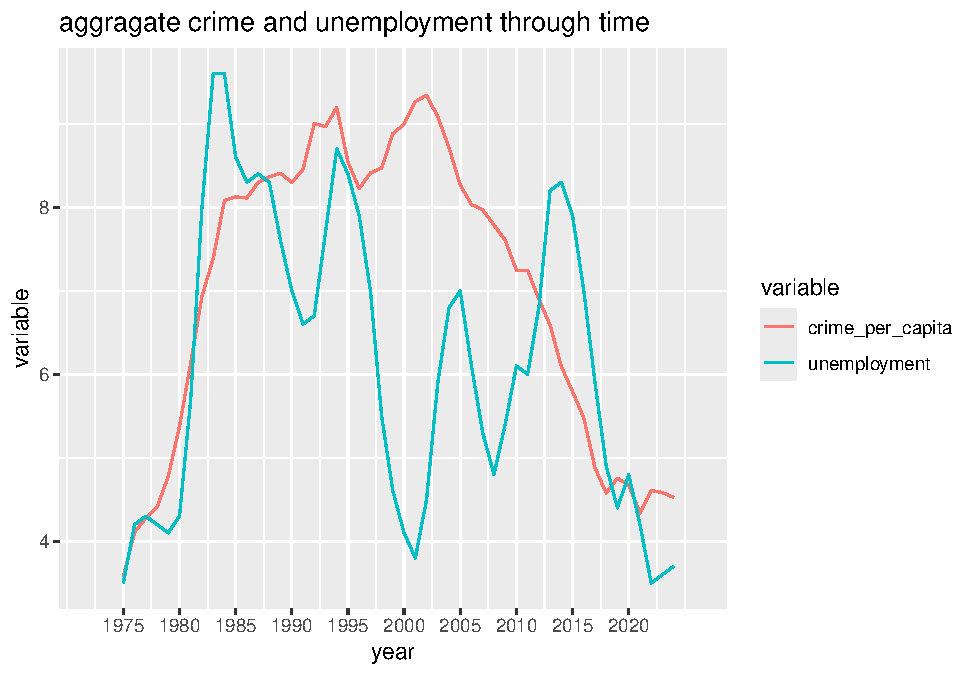
\includegraphics[keepaspectratio]{Template_Assignment_files/figure-latex/unnamed-chunk-4-1.pdf}}
This time series can be seperated into two larger periods. Pre 2000
where crime seems to follow unemployment, and post 2000 where crime
seems less corralated to unemployment, apart from certain periods.
Surprisingly, unemployment seems to be lagging behind crime in certain
periods.

\subsection{3.4 Visualize spatial
variation}\label{visualize-spatial-variation}

\begin{verbatim}
## 'data.frame':    620 obs. of  4 variables:
##  $ region: chr  "arbeidsmarktregio" "arbeidsmarktregio" "arbeidsmarktregio" "arbeidsmarktregio" ...
##  $ year  : int  2014 2015 2016 2017 2018 2019 2020 2021 2022 2023 ...
##  $ wgs84 : chr  "https://cartomap.github.io/nl/wgs84/arbeidsmarktregio_2014.geojson" "https://cartomap.github.io/nl/wgs84/arbeidsmarktregio_2015.geojson" "https://cartomap.github.io/nl/wgs84/arbeidsmarktregio_2016.geojson" "https://cartomap.github.io/nl/wgs84/arbeidsmarktregio_2017.geojson" ...
##  $ rd    : chr  "https://cartomap.github.io/nl/rd/arbeidsmarktregio_2014.geojson" "https://cartomap.github.io/nl/rd/arbeidsmarktregio_2015.geojson" "https://cartomap.github.io/nl/rd/arbeidsmarktregio_2016.geojson" "https://cartomap.github.io/nl/rd/arbeidsmarktregio_2017.geojson" ...
\end{verbatim}

\pandocbounded{\includegraphics[keepaspectratio]{Template_Assignment_files/figure-latex/unnamed-chunk-8-1.pdf}}

\pandocbounded{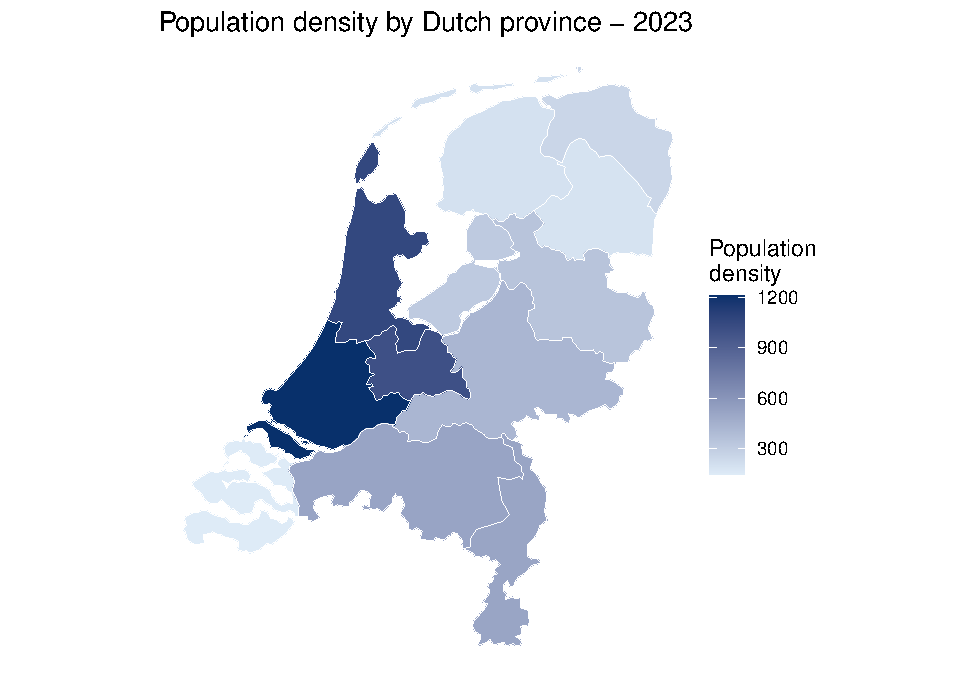
\includegraphics[keepaspectratio]{Template_Assignment_files/figure-latex/pop-heatmap-1.pdf}}

\pandocbounded{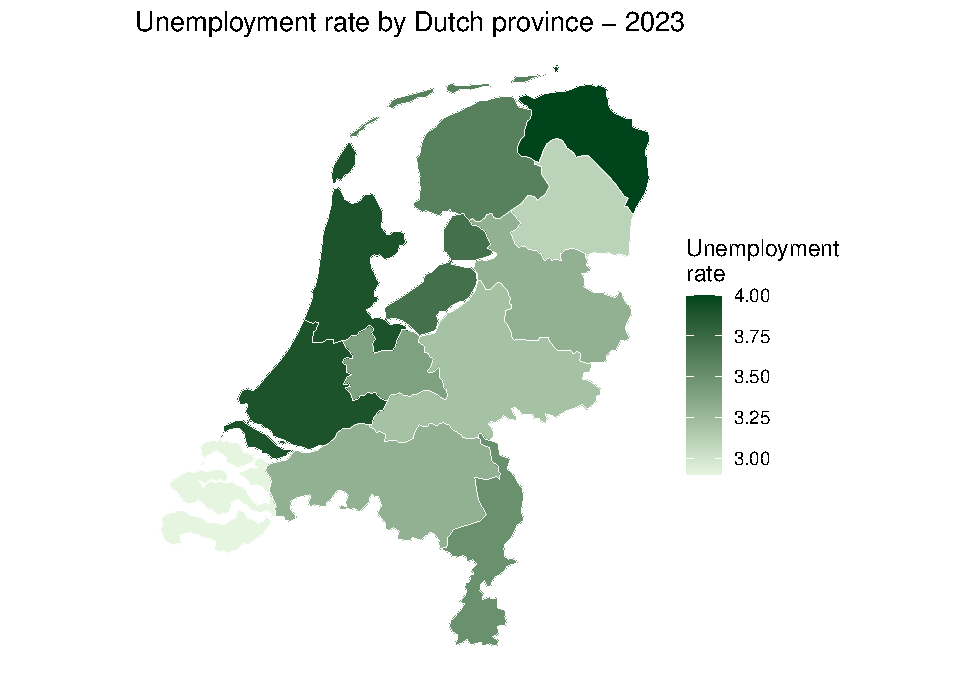
\includegraphics[keepaspectratio]{Template_Assignment_files/figure-latex/unemp-heatmap-1.pdf}}

\section{\textless\textless\textless\textless\textless\textless\textless{}
HEAD}\label{head}

We can generally see the pattern that crime per capita follows
unemployment. An anomaly is Groningen. Its unemployment is high, yet
crime per capita is failry low. Similarly, Flevoland's unemployment is
fairly yet its crime per capita is somewhat lower. If population density
is considered, than this pattern migh be better explained. Furthermore,
Other factors can also affect cause these anomalies, which shows that
the connection is not as straighforward. Individual cities and
munciplaties were not plotted, which impacts our abilitiy to draw
conclusions.

\begin{quote}
\begin{quote}
\begin{quote}
\begin{quote}
\begin{quote}
\begin{quote}
\begin{quote}
d22ac6077aa71c465abe179b2f0ae4d7a514a3ae \#\# 3.5 Visualize
sub-population variation
\end{quote}
\end{quote}
\end{quote}
\end{quote}
\end{quote}
\end{quote}
\end{quote}

\begin{Shaded}
\begin{Highlighting}[]
\FunctionTok{ggplot}\NormalTok{(crime2021, }\FunctionTok{aes}\NormalTok{(}\AttributeTok{x =}\NormalTok{ Age, }\AttributeTok{y =}\NormalTok{ Crime)) }\SpecialCharTok{+}
  \FunctionTok{geom\_boxplot}\NormalTok{(}\AttributeTok{fill =} \StringTok{"yellow"}\NormalTok{, }\AttributeTok{color =} \StringTok{"black"}\NormalTok{) }\SpecialCharTok{+}
  \FunctionTok{labs}\NormalTok{(}
    \AttributeTok{title =} \StringTok{"Boxplot of Crime Suspect Rate by Age Group in 2021"}\NormalTok{,}
    \AttributeTok{x =} \StringTok{"Age category"}\NormalTok{,}
    \AttributeTok{y =} \StringTok{"Crime Rate"}
\NormalTok{  ) }
\end{Highlighting}
\end{Shaded}

\pandocbounded{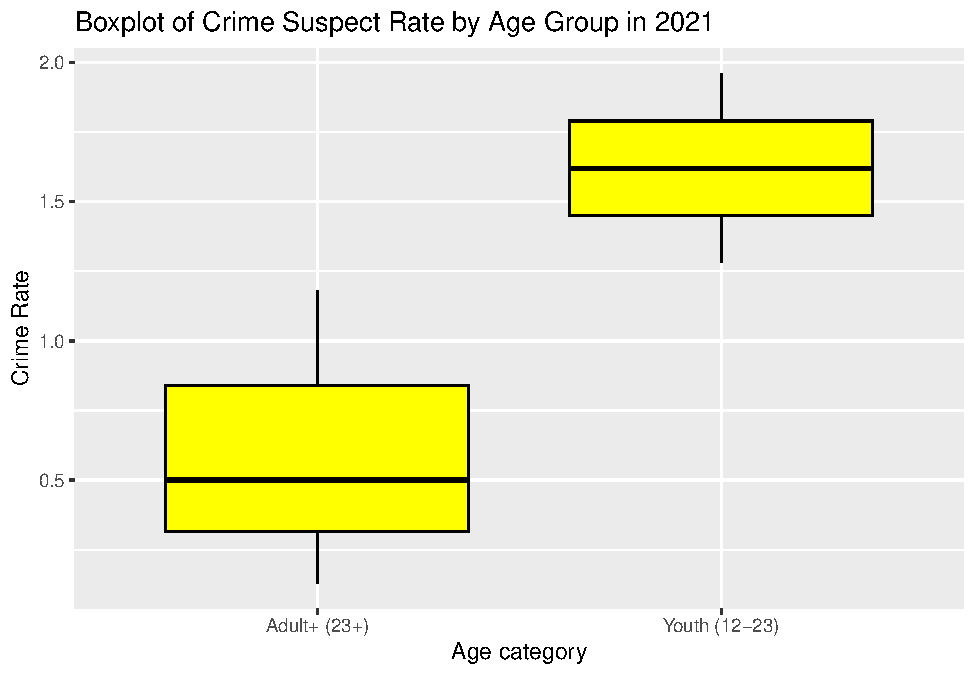
\includegraphics[keepaspectratio]{Template_Assignment_files/figure-latex/visualise_subpopulations-1.pdf}}

\begin{Shaded}
\begin{Highlighting}[]
\FunctionTok{ggplot}\NormalTok{(unemployment\_age, }\FunctionTok{aes}\NormalTok{(}\AttributeTok{x =}\NormalTok{ Age, }\AttributeTok{y =}\NormalTok{ Unemployment)) }\SpecialCharTok{+}
  \FunctionTok{geom\_boxplot}\NormalTok{(}\AttributeTok{fill =} \StringTok{"yellow"}\NormalTok{, }\AttributeTok{color =} \StringTok{"black"}\NormalTok{) }\SpecialCharTok{+}
  \FunctionTok{labs}\NormalTok{(}
    \AttributeTok{title =} \StringTok{"Boxplot of Crime Suspect Rate by Age Group in 2021"}\NormalTok{,}
    \AttributeTok{x =} \StringTok{"Age category"}\NormalTok{,}
    \AttributeTok{y =} \StringTok{"unemployment"}
\NormalTok{  ) }
\end{Highlighting}
\end{Shaded}

\pandocbounded{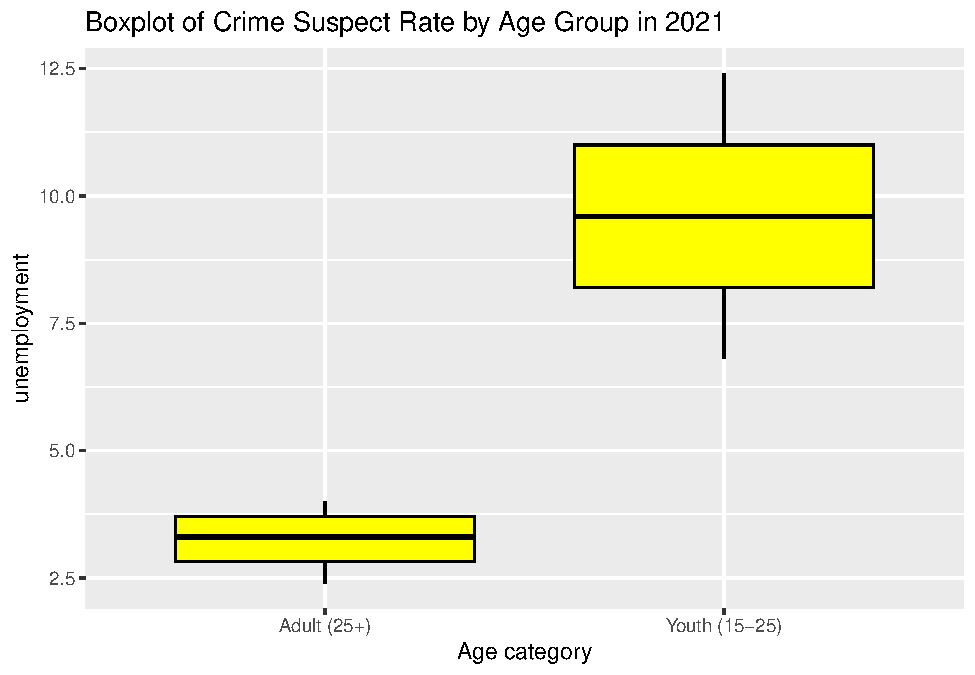
\includegraphics[keepaspectratio]{Template_Assignment_files/figure-latex/visualise_subpopulations-2.pdf}}

In the boxplots above, it is clearly visible that unemployment and crime
are linked. The Youth category is more vulnarable to unemployment than
the adult category (Yeung \& Yang, 2020), which in turn correlates with
higher crime rates. Kessler et al.~(2021) finds that reducing youth
unemployment reduces youth crimes. Data limitation limit causality
conclusions. Since the data does not distinguish if youth perpratrators
were unemployed. Furthermore, youth might also be more prone to
criminality regardless of employment status.

\subsection{3.6 Event analysis}\label{event-analysis}

\begin{Shaded}
\begin{Highlighting}[]
\NormalTok{pivot\_agg\_data }\OtherTok{\textless{}{-}}\NormalTok{ agg\_merged }\SpecialCharTok{\%\textgreater{}\%}
  \FunctionTok{pivot\_longer}\NormalTok{(}\AttributeTok{cols =} \FunctionTok{c}\NormalTok{(unemployment, crime\_per\_capita), }\AttributeTok{names\_to =} \StringTok{"variable"}\NormalTok{, }\AttributeTok{values\_to =} \StringTok{"value"}\NormalTok{)}

\FunctionTok{ggplot}\NormalTok{(pivot\_agg\_data, }\FunctionTok{aes}\NormalTok{(}\AttributeTok{x =}\NormalTok{ year, }\AttributeTok{y =}\NormalTok{ value, }\AttributeTok{colour =}\NormalTok{ variable )) }\SpecialCharTok{+}
  \FunctionTok{geom\_line}\NormalTok{() }\SpecialCharTok{+}
  \FunctionTok{labs}\NormalTok{(}\AttributeTok{title =} \StringTok{"aggragate crime and unemployment through time"}\NormalTok{, }\AttributeTok{x =} \StringTok{"year"}\NormalTok{, }\AttributeTok{y =} \StringTok{"variable"}\NormalTok{) }\SpecialCharTok{+}
  \FunctionTok{scale\_x\_continuous}\NormalTok{(}\AttributeTok{breaks =} \FunctionTok{seq}\NormalTok{(}\DecValTok{1975}\NormalTok{, }\DecValTok{2024}\NormalTok{, }\AttributeTok{by =} \DecValTok{5}\NormalTok{), }\AttributeTok{limits =} \FunctionTok{c}\NormalTok{(}\DecValTok{1972}\NormalTok{, }\DecValTok{2026}\NormalTok{)) }\SpecialCharTok{+}
  \FunctionTok{geom\_vline}\NormalTok{(}\AttributeTok{xintercept =} \FunctionTok{c}\NormalTok{(}\DecValTok{1979}\NormalTok{, }\DecValTok{2008}\NormalTok{), }
             \AttributeTok{linetype =} \StringTok{"solid"}\NormalTok{, }
             \AttributeTok{color =} \StringTok{"black"}\NormalTok{, }
             \AttributeTok{linewidth =} \FloatTok{0.6}\NormalTok{) }\SpecialCharTok{+} 
  \FunctionTok{annotate}\NormalTok{(}\StringTok{"text"}\NormalTok{, }\AttributeTok{x =} \DecValTok{1974}\NormalTok{, }\AttributeTok{y =} \DecValTok{9}\NormalTok{, }\AttributeTok{label =} \StringTok{"1979}\SpecialCharTok{\textbackslash{}n}\StringTok{oil{-}crisis"}\NormalTok{) }\SpecialCharTok{+}
  \FunctionTok{annotate}\NormalTok{(}\StringTok{"text"}\NormalTok{, }\AttributeTok{x =} \DecValTok{2017}\NormalTok{, }\AttributeTok{y =} \DecValTok{9}\NormalTok{, }\AttributeTok{label =} \StringTok{"2008}\SpecialCharTok{\textbackslash{}n}\StringTok{great{-}recession"}\NormalTok{)}
\end{Highlighting}
\end{Shaded}

\pandocbounded{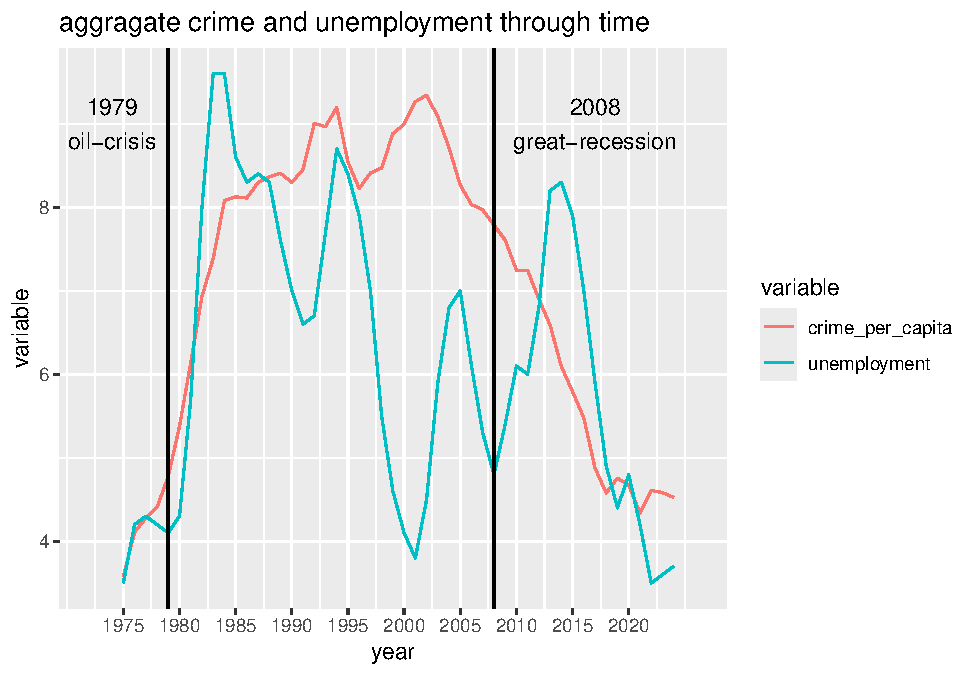
\includegraphics[keepaspectratio]{Template_Assignment_files/figure-latex/analysis-1.pdf}}

Both 1979 oil-crises and the 2008 recession see large spikes in
unemployment, yet only 1979 sees an increase in crimp per capita as
well. A possible explanation for the movement of crime per capita in
accordance with unemployment in 1980 to an inverse movement in 2008
could be the fact that the population is much younger in 1980 compared
to 2008 and thus more people are in their peak-crime committing age
18-35 (Bezuinigen En Hervormingen in De Jaren '80, 2022). Another
explanation is that the welfare safety net was much more robust in 2008
than in the 1980's which means that people who were unemployed where
less inclined to do crime (Bezuinigen En Hervormingen in De Jaren '80,
2022). This shows that while unemployment may be linked in some cases,
other factors play a significant role as well. Furthermore, trends in
crime per capita predates trends in unemployment during both events,
which negatively impacts the validity of our conclusions.

\section{Part 4 - Discussion}\label{part-4---discussion}

\subsection{4.1 Discuss your findings}\label{discuss-your-findings}

The results clearly shows that unemployment and crime are correlated,
but also implicates that there is not a direct causality between
unemployment and crime. Unemployment is likely a catalyst for crime.
That is, unemployment is related to various social factors which might
directly impact potency to commit crimes. These results can be of
interest for policy makers, as not only battling unemployment helps
prevent crime, but setting up other social programs might reduce
blowbacks of unemployment. Allocating funds towards vulnarable groups,
such as youth, and areas with a high population density will achieve the
greatest results.

\section{Part 5 - Reproducibility}\label{part-5---reproducibility}

\subsection{5.1 Github repository link}\label{github-repository-link}

Provide the link to your PUBLIC repository
here:\url{https://github.com/Autelius/Crime-and-Unemployment-Group-Project-FR-GIT.git}

\subsection{5.2 Reference list}\label{reference-list}

Fischer, T. (2015). De relatie tussen werk en criminaliteit uitgeplozen.
Tijdschrift voor Criminologie, 57(3), 334--338.
\url{https://www.boomportaal.nl/tijdschrift/TvC/TvC_0165-182X_2015_057_003_008}

Nieuws Sociaal en Groen. (2023). Criminaliteit: de stand van zaken in
Nederland. Retrieved from
\url{https://nieuwsociaalengroen.nl/criminaliteit/}

Verbruggen, J. (2014). Previously institutionalized youths on the road
to adulthood: A longitudinal study on employment and crime.
{[}PhD-Thesis - Research and graduation internal, Vrije Universiteit
Amsterdam{]}.

Statline. (2025). Arbeidsdeelname; provincie, 2013--2024 {[}Data set{]}.
Centraal Bureau voor de Statistiek.
\url{https://opendata.cbs.nl/\#/CBS/nl/dataset/85268NED/table?dl=BE1FB}

Cbs. (2025). Geregistreerde criminaliteit; soort misdrijf, regio,
2010-2024 {[}Data set{]}. Centraal Bureau voor de Statistiek.
\url{https://opendata.cbs.nl/\#/CBS/nl/dataset/85268NED/table?dl=BE1FB}

Statline. (2025). Bevolkingsontwikkeling; regio per maand, 2002-2024
{[}Data set{]}. Centraal Bureau voor de Statistiek.
\url{https://opendata.cbs.nl/\#/CBS/nl/dataset/37230ned/table}

Statline. (2006). Volkstelling; oppervlakten, 1930 {[}Data set{]}.
Centraal Bureau voor de Statistiek.
\url{https://opendata.cbs.nl/\#/CBS/nl/dataset/71118NED/table}

Statline. (2025). Geregistreerde criminaliteit, 1948-2024 {[}Data
set{]}. Centraal Bureau voor de Statistiek.
\url{https://opendata.cbs.nl/\#/CBS/nl/dataset/83723NED/table}

Statline. (2025). Verdachten; geslacht, leeftijd, herkomst, opleiding,
huishoudensinkomen, 2010-2024 {[}Data set{]}. Centraal Bureau voor de
Statistiek.
\url{https://opendata.cbs.nl/\#/CBS/nl/dataset/85658NED/table}

Statline. (2025). Arbeidsdeelname; kerncijfers, 2013-2024 {[}Data
set{]}. Centraal Bureau voor de Statistiek.
\url{https://opendata.cbs.nl/\#/CBS/nl/dataset/85264NED/table?dl=BE1F8}

Bezuinigen en hervormingen in de jaren '80. (2022, June 21).
IsGeschiedenis.
\url{https://isgeschiedenis.nl/nieuws/bezuinigen-en-hervormingen-in-de-jaren-80}

Yeung, W. J., \& Yang, Y. (2020). Labor Market Uncertainties for Youth
and Young Adults: An International Perspective. The Annals Of The
American Academy Of Political And Social Science, 688(1), 7--19.
\url{https://doi.org/10.1177/0002716220913487}

Kessler, J. B., Tahamont, S., Gelber, A., \& Isen, A. (2022). The
Effects of Youth Employment on Crime: Evidence from New York City
Lotteries. Journal Of Policy Analysis And Management, 41(3), 710--730.
\url{https://doi.org/10.1002/pam.22393}

\end{document}
